\section{Graphics\-Data Struct Reference}
\label{structGraphicsData}\index{GraphicsData@{GraphicsData}}
{\tt \#include $<$system.hpp$>$}

Collaboration diagram for Graphics\-Data:\begin{figure}[H]
\begin{center}
\leavevmode
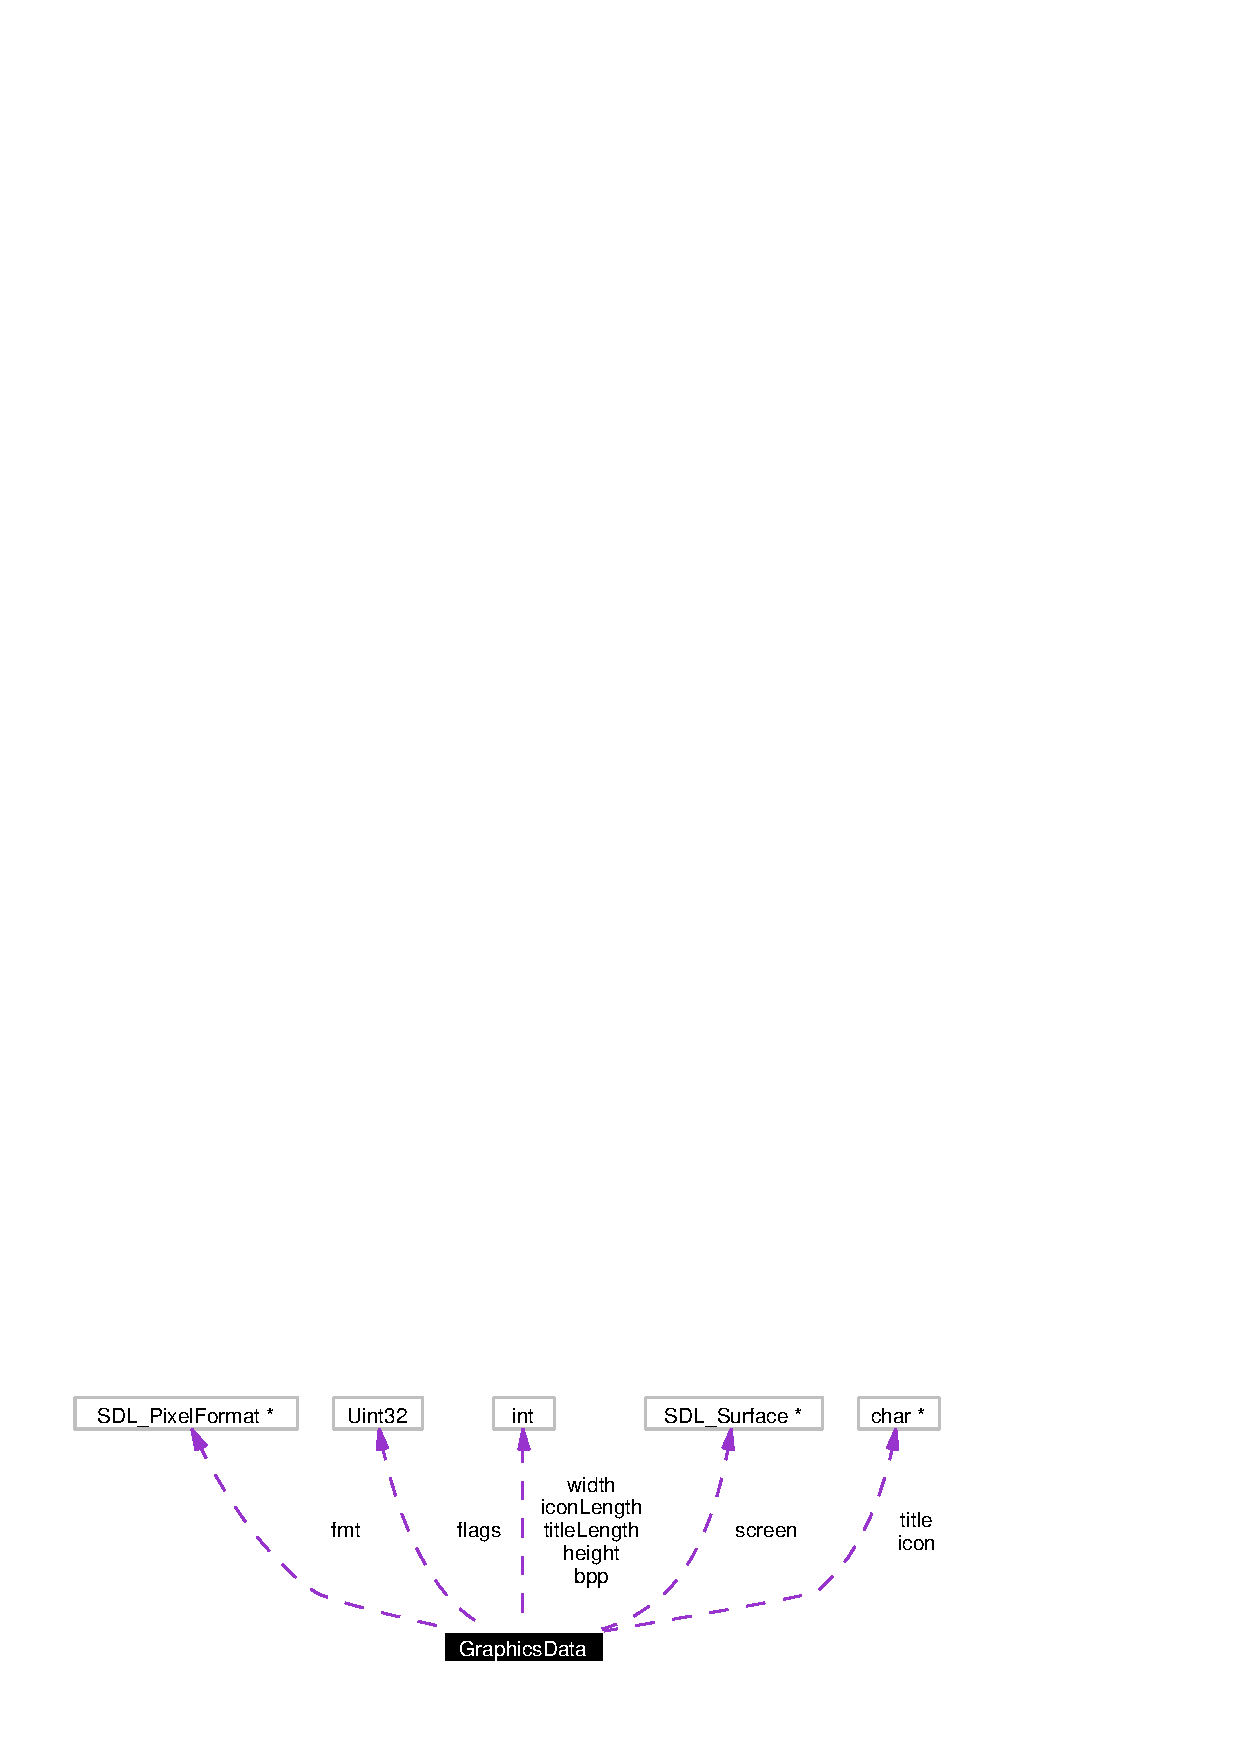
\includegraphics[width=231pt]{structGraphicsData__coll__graph}
\end{center}
\end{figure}
\subsection*{Public Attributes}
\begin{CompactItemize}
\item 
SDL\_\-Surface $\ast$ {\bf screen}
\item 
SDL\_\-Pixel\-Format $\ast$ {\bf fmt}
\item 
int {\bf width}
\item 
int {\bf height}
\item 
int {\bf bpp}
\item 
Uint32 {\bf flags}
\item 
char $\ast$ {\bf title}
\item 
char $\ast$ {\bf icon}
\item 
int {\bf title\-Length}
\item 
int {\bf icon\-Length}
\end{CompactItemize}


\subsection{Member Data Documentation}
\index{GraphicsData@{Graphics\-Data}!bpp@{bpp}}
\index{bpp@{bpp}!GraphicsData@{Graphics\-Data}}
\subsubsection{\setlength{\rightskip}{0pt plus 5cm}int {\bf Graphics\-Data::bpp}}\label{structGraphicsData_o4}


\index{GraphicsData@{Graphics\-Data}!flags@{flags}}
\index{flags@{flags}!GraphicsData@{Graphics\-Data}}
\subsubsection{\setlength{\rightskip}{0pt plus 5cm}Uint32 {\bf Graphics\-Data::flags}}\label{structGraphicsData_o5}


\index{GraphicsData@{Graphics\-Data}!fmt@{fmt}}
\index{fmt@{fmt}!GraphicsData@{Graphics\-Data}}
\subsubsection{\setlength{\rightskip}{0pt plus 5cm}SDL\_\-Pixel\-Format$\ast$ {\bf Graphics\-Data::fmt}}\label{structGraphicsData_o1}


\index{GraphicsData@{Graphics\-Data}!height@{height}}
\index{height@{height}!GraphicsData@{Graphics\-Data}}
\subsubsection{\setlength{\rightskip}{0pt plus 5cm}int {\bf Graphics\-Data::height}}\label{structGraphicsData_o3}


\index{GraphicsData@{Graphics\-Data}!icon@{icon}}
\index{icon@{icon}!GraphicsData@{Graphics\-Data}}
\subsubsection{\setlength{\rightskip}{0pt plus 5cm}char$\ast$ {\bf Graphics\-Data::icon}}\label{structGraphicsData_o7}


\index{GraphicsData@{Graphics\-Data}!iconLength@{iconLength}}
\index{iconLength@{iconLength}!GraphicsData@{Graphics\-Data}}
\subsubsection{\setlength{\rightskip}{0pt plus 5cm}int {\bf Graphics\-Data::icon\-Length}}\label{structGraphicsData_o9}


\index{GraphicsData@{Graphics\-Data}!screen@{screen}}
\index{screen@{screen}!GraphicsData@{Graphics\-Data}}
\subsubsection{\setlength{\rightskip}{0pt plus 5cm}SDL\_\-Surface$\ast$ {\bf Graphics\-Data::screen}}\label{structGraphicsData_o0}


\index{GraphicsData@{Graphics\-Data}!title@{title}}
\index{title@{title}!GraphicsData@{Graphics\-Data}}
\subsubsection{\setlength{\rightskip}{0pt plus 5cm}char$\ast$ {\bf Graphics\-Data::title}}\label{structGraphicsData_o6}


\index{GraphicsData@{Graphics\-Data}!titleLength@{titleLength}}
\index{titleLength@{titleLength}!GraphicsData@{Graphics\-Data}}
\subsubsection{\setlength{\rightskip}{0pt plus 5cm}int {\bf Graphics\-Data::title\-Length}}\label{structGraphicsData_o8}


\index{GraphicsData@{Graphics\-Data}!width@{width}}
\index{width@{width}!GraphicsData@{Graphics\-Data}}
\subsubsection{\setlength{\rightskip}{0pt plus 5cm}int {\bf Graphics\-Data::width}}\label{structGraphicsData_o2}




The documentation for this struct was generated from the following file:\begin{CompactItemize}
\item 
src/{\bf system.hpp}\end{CompactItemize}
